\chapter{Results and Discussion}
\label{ch:results}

This chapter reports the results of the four models described in \cref{ch:method}, evaluated as set out in \cref{ch:setup}. Every value in this chapter is taken from the saved result files and console logs listed in \cref{app:repro}. Each configuration was trained once, so differences between models are differences between single runs; this is taken into account in the discussion.

\section{Overall Experimental Results}
\label{sec:overall}

\Cref{tab:main} gives the accuracy of each model on its validation split and on the shared held-out test split of 478 scenarios from 200- to 300-node topologies. \Cref{fig:ood-bar} shows the test results graphically.

\begin{table}[ht]
\centering
\small
\caption{Accuracy of all models. Test MAPE is measured on the same 478 held-out scenarios (200--300 nodes) for every model. Validation MAPE is on each model's own validation split and is not comparable between the baseline and the other models.}
\label{tab:main}
\begin{tabular}{@{}l l c c c@{}}
\toprule
\textbf{Model} & \textbf{Architecture} & \textbf{Training topologies} & \textbf{Validation MAPE (\%)} & \textbf{Test MAPE (\%)} \\
\midrule
Baseline        & RouteNet-Fermi    & 10 nodes       & 6.41$^{a}$ & 8.40 \\
Teacher         & RouteNet-Fermi    & 10--170 nodes  & 4.71       & \textbf{5.37} \\
Student-scratch & Queue-Link Fusion & 10--170 nodes  & 10.65      & 11.92 \\
Student-KD      & Queue-Link Fusion & 10--170 nodes  & 9.04$^{b}$ & 9.83 \\
\bottomrule
\end{tabular}

\vspace{1mm}
\begin{minipage}{0.95\textwidth}
\footnotesize
$^{a}$Original validation split: 25 scenarios from five topologies of 100--300 nodes. Value recorded at the selected epoch during training.\\
$^{b}$Flow-weighted MAPE from evaluating the saved checkpoint. The unweighted value recorded during training was 9.64 (\cref{sec:kd-discrepancy}).
\end{minipage}
\end{table}

\begin{figure}[ht]
\centering
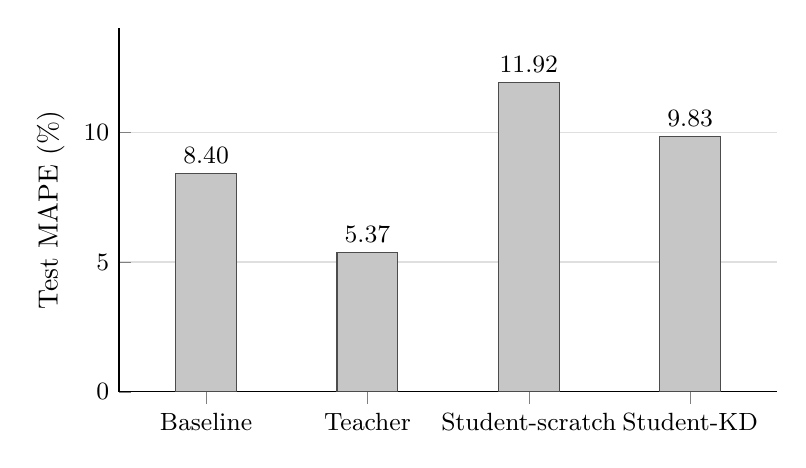
\begin{tikzpicture}
\begin{axis}[
  ybar,
  width=0.82\textwidth,
  height=6.2cm,
  bar width=22pt,
  ymin=0, ymax=14,
  ylabel={Test MAPE (\%)},
  symbolic x coords={Baseline,Teacher,Student-scratch,Student-KD},
  xtick=data,
  nodes near coords={\pgfmathprintnumber[fixed,fixed zerofill,precision=2]{\pgfplotspointmeta}},
  nodes near coords style={font=\small},
  axis lines*=left,
  ymajorgrids=true,
  grid style={gray!25},
  enlarge x limits=0.18,
  tick label style={font=\small},
]
\addplot[fill=gray!45, draw=black!70] coordinates {
  (Baseline,8.4011) (Teacher,5.3734) (Student-scratch,11.9244) (Student-KD,9.8280)
};
\end{axis}
\end{tikzpicture}
\caption{MAPE on the held-out 200--300-node test set (478 scenarios) for each model.}
\label{fig:ood-bar}
\end{figure}

Three results stand out.

\paragraph{The topology-diverse teacher is the most accurate model.} On the held-out test set the teacher's MAPE is 5.37\%, against 8.40\% for the baseline. This is a reduction of 3.03 percentage points, or 36.0\% in relative terms. The two models have identical architectures and start from the same initial weights; they differ in the training data, in the amount of training (\cref{sec:discussion}) and in the data used to select the checkpoint.

\paragraph{The compressed student loses accuracy.} Trained on the same data as the teacher but without distillation, the student reaches 11.92\% test MAPE, which is 2.22 times the teacher's error. Its validation MAPE (10.65\%) is similarly about 2.3 times the teacher's (4.71\%).

\paragraph{Distillation improves the student.} With distillation, the student's test MAPE falls from 11.92\% to 9.83\%, a reduction of 2.10 percentage points or 17.6\% in relative terms. On the validation split, MAPE falls from 10.65\% to 9.04\% (1.60 points, 15.0\%). The distilled student remains less accurate than both full-size models: its test MAPE is 4.45 points above the teacher's and 1.43 points above the baseline's.

\subsection{Training behaviour}

\Cref{fig:curves} shows the validation curves recorded during training. The teacher's validation MAPE (\cref{fig:curve-teacher}) fluctuates considerably from epoch to epoch, between 4.71\% and 6.76\% after epoch 10, even though its training loss decreases steadily. The fluctuation reflects the composition of the validation split, which holds a single topology of each size, so a change in how well the model fits one topology can move the overall value noticeably. The distillation run (\cref{fig:curve-kd}) is much smoother: its validation loss decreases almost monotonically until about epoch 15 and then levels off around 9.6--9.7\% before early stopping ends training at epoch 24. The baseline's validation curve (\cref{app:logs}) is as erratic as the teacher's, with values between 6.41\% and 8.35\% across its 15 epochs; its selected checkpoint is the last epoch, so it is possible that further training would have changed the result.

\begin{figure}[ht]
\centering
\begin{subfigure}[b]{0.49\textwidth}
\centering
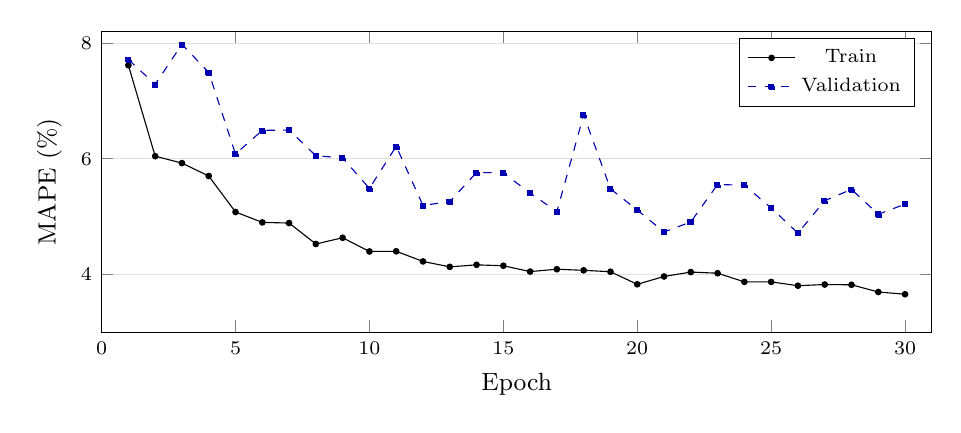
\begin{tikzpicture}
\begin{axis}[
  width=\textwidth, height=5.4cm,
  xlabel={Epoch}, ylabel={MAPE (\%)},
  xmin=0, xmax=31, ymin=3, ymax=8.2,
  legend style={font=\scriptsize, at={(0.98,0.98)}, anchor=north east},
  tick label style={font=\scriptsize}, label style={font=\small},
  ymajorgrids=true, grid style={gray!25},
]
\addplot[black, mark=*, mark size=1pt] coordinates {
(1,7.6173)(2,6.0447)(3,5.9251)(4,5.7016)(5,5.0794)(6,4.8996)(7,4.8883)(8,4.5263)(9,4.6338)(10,4.3966)
(11,4.3999)(12,4.2246)(13,4.1303)(14,4.1656)(15,4.1494)(16,4.0491)(17,4.0895)(18,4.0708)(19,4.0458)(20,3.8289)
(21,3.9641)(22,4.0405)(23,4.0208)(24,3.8710)(25,3.8707)(26,3.8044)(27,3.8249)(28,3.8205)(29,3.6957)(30,3.6569)};
\addlegendentry{Train}
\addplot[blue!70!black, dashed, mark=square*, mark size=1pt] coordinates {
(1,7.7157)(2,7.2879)(3,7.9793)(4,7.4936)(5,6.0834)(6,6.4913)(7,6.4972)(8,6.0524)(9,6.0155)(10,5.4865)
(11,6.2160)(12,5.1928)(13,5.2589)(14,5.7631)(15,5.7563)(16,5.4061)(17,5.0863)(18,6.7599)(19,5.4792)(20,5.1151)
(21,4.7331)(22,4.9076)(23,5.5545)(24,5.5437)(25,5.1506)(26,4.7139)(27,5.2744)(28,5.4711)(29,5.0402)(30,5.2150)};
\addlegendentry{Validation}
\end{axis}
\end{tikzpicture}
\caption{Teacher (best epoch 26).}
\label{fig:curve-teacher}
\end{subfigure}
\hfill
\begin{subfigure}[b]{0.49\textwidth}
\centering
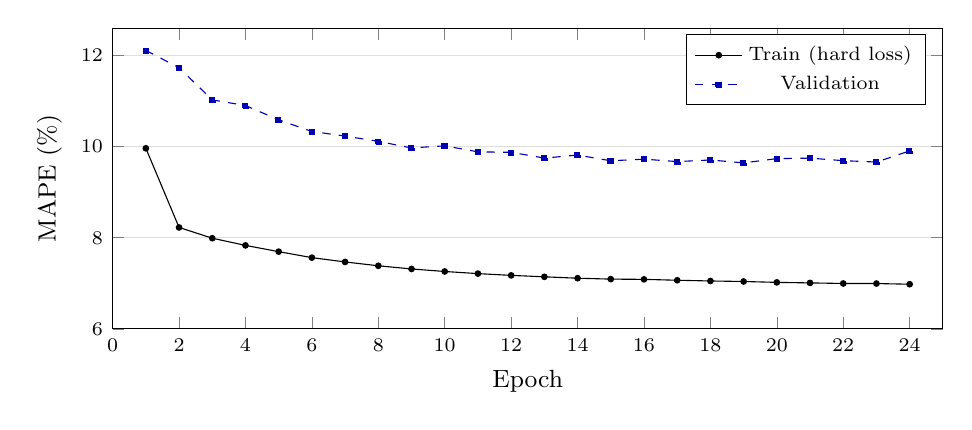
\begin{tikzpicture}
\begin{axis}[
  width=\textwidth, height=5.4cm,
  xlabel={Epoch}, ylabel={MAPE (\%)},
  xmin=0, xmax=25, ymin=6, ymax=12.6,
  legend style={font=\scriptsize, at={(0.98,0.98)}, anchor=north east},
  tick label style={font=\scriptsize}, label style={font=\small},
  ymajorgrids=true, grid style={gray!25},
]
\addplot[black, mark=*, mark size=1pt] coordinates {
(1,9.9645)(2,8.2266)(3,7.9904)(4,7.8328)(5,7.6954)(6,7.5641)(7,7.4693)(8,7.3852)(9,7.3156)(10,7.2600)
(11,7.2133)(12,7.1745)(13,7.1431)(14,7.1124)(15,7.0925)(16,7.0871)(17,7.0677)(18,7.0516)(19,7.0404)(20,7.0209)
(21,7.0095)(22,6.9965)(23,6.9952)(24,6.9804)};
\addlegendentry{Train (hard loss)}
\addplot[blue!70!black, dashed, mark=square*, mark size=1pt] coordinates {
(1,12.1137)(2,11.7319)(3,11.0272)(4,10.9029)(5,10.5883)(6,10.3335)(7,10.2322)(8,10.1161)(9,9.9722)(10,10.0181)
(11,9.8867)(12,9.8760)(13,9.7496)(14,9.8157)(15,9.6898)(16,9.7258)(17,9.6723)(18,9.7076)(19,9.6439)(20,9.7374)
(21,9.7480)(22,9.6928)(23,9.6622)(24,9.9065)};
\addlegendentry{Validation}
\end{axis}
\end{tikzpicture}
\caption{Student-KD (best epoch 19).}
\label{fig:curve-kd}
\end{subfigure}
\caption{Per-epoch MAPE recorded during training. For the student-KD run, both curves are unweighted means over scenarios (\cref{sec:metrics}), and the training curve shows only the hard (ground-truth) term of the loss.}
\label{fig:curves}
\end{figure}

\section{Comparison with Existing Methods}
\label{sec:comparison}

The existing method against which this work is compared is RouteNet-Fermi itself, represented by the baseline (trained according to the reference implementation's few-shot script on the original 10-node training data) and by the teacher (the same architecture trained on topology-diverse data). Published RouteNet-Fermi figures are not quoted for comparison because they were obtained with a different training budget and evaluation protocol, and the aim here is a like-for-like comparison on one test set.

For completeness, \cref{tab:hist} also records the baseline's results on the dataset's original test split, which spans 50 to 300 nodes and therefore includes topologies that were later moved into the teacher's training data. These numbers are not comparable with the teacher and student results, but they show that the baseline's error on the 200- to 300-node subset (8.40\%) is similar to its error on the full original test set (8.22\%) with the same checkpoint. The first training run, selected at epoch 3, gave a higher error of 9.17\% on the original test split, which illustrates how much a single run and the choice of checkpoint can move the result.

\begin{table}[ht]
\centering
\small
\caption{Baseline results on the two test sets. Only the last row is comparable with the teacher and student results in \cref{tab:main}.}
\label{tab:hist}
\begin{tabular}{@{}l l c c@{}}
\toprule
\textbf{Run (checkpoint)} & \textbf{Test set} & \textbf{Scenarios} & \textbf{MAPE (\%)} \\
\midrule
Run 1 (epoch 3)  & Original test, 50--300 nodes   & 878 & 9.17 \\
Run 2 (epoch 15) & Original test, 50--300 nodes   & 878 & 8.22 \\
Run 2 (epoch 15) & Held-out test, 200--300 nodes  & 478 & 8.40 \\
\bottomrule
\end{tabular}
\end{table}

Other classes of method discussed in \cref{ch:related}, such as queueing-theory models, packet simulation and graph-free distilled students, were not run in this project, so no quantitative comparison with them is claimed.

\section{Additional Analyses}
\label{sec:analyses}

\subsection{Model size and inference latency}
\label{sec:efficiency}

\Cref{tab:efficiency} reports the efficiency measurements. The student has 83.3\% fewer trainable parameters than RouteNet-Fermi (4,505 against 27,025, a ratio of 6.0), its weights occupy 17.6~KB against 105.6~KB, and it performs one third of the message-passing stages. A single forward pass on the benchmark scenario took 34.2~ms on average for the student, against 178.5~ms for the teacher and 177.5~ms for the baseline, making the student about 5.2 times faster. The student's latency was also much more stable, with a standard deviation of 1.8~ms against 9.4--13.0~ms for the full-size models. The baseline and teacher, which share an architecture, have the same latency within measurement noise, as expected.

\begin{table}[ht]
\centering
\small
\caption{Model size and single-forward-pass latency on CPU (30 timed runs after 5 warm-up runs, one validation scenario). Student-KD shares the student architecture and was not timed separately.}
\label{tab:efficiency}
\begin{tabular}{@{}l r r c c c c c@{}}
\toprule
\multirow{2}{*}{\textbf{Model}} & \multirow{2}{*}{\textbf{Params}} & \multirow{2}{*}{\textbf{Size (KB)}} & \multirow{2}{*}{\textbf{MP stages}} & \multicolumn{3}{c}{\textbf{Latency (ms)}} & \multirow{2}{*}{\textbf{Speed-up}} \\
\cmidrule(lr){5-7}
 & & & & Mean & Median & Std & \\
\midrule
Baseline        & 27,025 & 105.6 & 24 & 177.5 & 175.5 & 13.0 & 1.01$\times$ \\
Teacher         & 27,025 & 105.6 & 24 & 178.5 & 177.6 & 9.4  & 1.00$\times$ \\
Student-scratch & 4,505  & 17.6  & 8  & 34.2  & 33.9  & 1.8  & 5.22$\times$ \\
Student-KD      & 4,505  & 17.6  & 8  & \multicolumn{3}{c}{not measured} & --- \\
\bottomrule
\end{tabular}
\end{table}

\Cref{fig:tradeoff} places the four models on a plane of test error against model size. No model is better than the others on both axes. The teacher gives the lowest error at full size; the distilled student gives the lowest error among the small models.

\begin{figure}[ht]
\centering
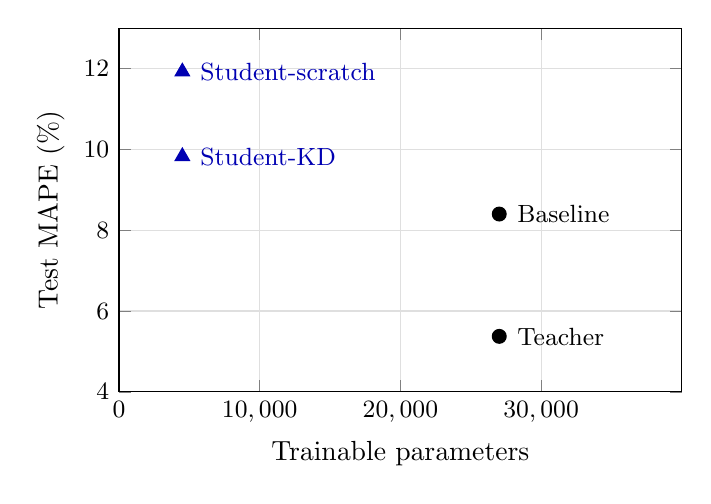
\begin{tikzpicture}
\begin{axis}[
  width=0.72\textwidth, height=6.2cm,
  xlabel={Trainable parameters}, ylabel={Test MAPE (\%)},
  xmin=0, xmax=40000, ymin=4, ymax=13,
  xtick={0,10000,20000,30000},
  clip=false,
  scaled x ticks=false,
  xticklabel style={/pgf/number format/.cd, fixed, 1000 sep={,}},
  ymajorgrids=true, xmajorgrids=true, grid style={gray!25},
  tick label style={font=\small},
  nodes near coords, point meta=explicit symbolic,
  nodes near coords style={font=\small, anchor=west, xshift=3pt},
]
\addplot[only marks, mark=*, mark size=2.5pt] coordinates {
  (27025,8.4011) [Baseline]
  (27025,5.3734) [Teacher]
};
\addplot[only marks, mark=triangle*, mark size=3pt, blue!70!black] coordinates {
  (4505,11.9244) [Student-scratch]
  (4505,9.8280) [Student-KD]
};
\end{axis}
\end{tikzpicture}
\caption{Test MAPE against number of trainable parameters. Circles: RouteNet-Fermi; triangles: Queue-Link Fusion.}
\label{fig:tradeoff}
\end{figure}

\subsection{End-to-end evaluation time}

The forward-pass benchmark excludes reading the scenario and building its graph. The evaluation logs give a complementary view of total processing time on the large test topologies. Evaluating the 478 test scenarios took 9,307~s for the baseline, 9,642~s for the teacher, 8,938~s for student-scratch and 9,032~s for student-KD, which is roughly 19--20~s per scenario for every model. Since a fivefold difference in forward-pass cost changed the total by only about 7\%, most of the per-scenario time in this pipeline is spent outside the model. The pipeline was not profiled, but the likely candidates are parsing the simulator output and building the graph with NetworkX in Python. The student's speed advantage is therefore real for the model itself, but a deployment would also need a faster graph-construction step to benefit from it fully.

\subsection{Generalisation gap}

For the three models trained on the topology-diverse split, the difference between test and validation MAPE indicates how much accuracy is lost when moving from topologies of up to 170 nodes to topologies of 200 to 300 nodes. The gap is 0.66 points for the teacher (4.71\% to 5.37\%), 1.28 points for student-scratch (10.65\% to 11.92\%) and 0.78 points for student-KD (9.04\% to 9.83\%). The distilled student's gap is closer to the teacher's than to that of the student trained from scratch. This is consistent with the student having absorbed some of the teacher's behaviour on larger topologies, although with a single run per model the difference between 0.78 and 1.28 points cannot be treated as established.

\subsection{Validation metric discrepancy in the distillation run}
\label{sec:kd-discrepancy}

The distillation training run recorded a best validation MAPE of 9.64\% at epoch 19, but evaluating the saved epoch-19 checkpoint afterwards gave 9.04\% on the same validation split. The saved checkpoint is the one written at epoch 19 (the evaluation log loads \texttt{ckpt-19}), so the difference is not due to loading the wrong weights. The likely cause is the aggregation difference described in \cref{sec:metrics}. The custom validation step in the distillation loop averages per-scenario MAPE with equal weight per scenario, while Keras's \texttt{evaluate} weights each scenario by its number of flows. Larger topologies contain many more flows, so a lower flow-weighted value means that the student is more accurate, in relative terms, on the larger validation topologies than on the smaller ones. This explanation follows from the code; it has not been confirmed by recomputing both aggregates from saved per-scenario predictions.

Two consequences follow. First, the 9.04\% figure is the one comparable with all other validation values in this report, which were obtained through the same Keras routines. Second, the distillation run selected its checkpoint with a slightly different criterion from the other runs. With the per-scenario curve flat between epochs 15 and 23 (\cref{fig:curve-kd}), a flow-weighted criterion might have selected a different epoch, but the difference is unlikely to be large.

\subsection{Relative size of the distillation loss terms}

At the selected epoch of the distillation run, the mean training values of the two terms in \cref{eq:kd} were 7.04 for the hard MAPE term and 0.169 for the soft MSE term, giving a total of $0.5 \times 7.04 + 0.5 \times 0.169 = 3.60$, which matches the logged total of 3.6045. The soft term therefore made up only about 2.3\% of the loss value. This does not mean that the teacher signal had a negligible effect, because what matters for training is the gradient of each term and Adam rescales update magnitudes, but it does mean that $\alpha = 0.5$ should not be read as an even split of influence between the ground truth and the teacher. The MSE is computed on raw delay values, which are small for most flows and large for a few, so the soft term is likely to be dominated by the flows with the longest delays.

\section{Discussion of Findings}
\label{sec:discussion}

\subsection{Topology diversity and the full-size models}

The clearest result is that the teacher, trained on topologies of up to 170 nodes, is substantially more accurate on 200- to 300-node topologies than the baseline trained only on 10-node topologies. Learning delay behaviour on larger networks, with longer paths and more flows sharing each link, appears to transfer better to even larger networks than learning it on very small ones. This finding is relevant beyond this project: when preparing training data for a learned network model, including topologies closer in size to the target deployment is likely to help more than additional samples from small topologies.

The comparison is not perfectly controlled, however. The teacher was trained for about 299,000 steps ($30 \times 9{,}972$), while the baseline followed the reference few-shot script with 37,500 steps ($15 \times 2{,}500$), about one eighth as many. The baseline's best checkpoint was its last, so it may not have converged. Part of the teacher's advantage could therefore come from longer training rather than from the more diverse data. A baseline trained on 10-node data for the same number of steps would separate the two effects.

\subsection{The cost of compression}

The scratch student's error is 2.2 times the teacher's, so the compression in its current form has a significant accuracy cost. Several features of the design may contribute, and the results do not identify which matters most.
\begin{itemize}
  \item \textbf{Loss of per-queue information.} As explained in \cref{sec:fusion-cost}, a flow in the student sees the average state of all queues on a link, not the state of the queue it actually uses, and the flow features do not include its ToS class. Under strict-priority and weighted scheduling, flows of different classes on the same link can have very different delays, and the student has no direct way to distinguish them.
  \item \textbf{Fewer message-passing iterations.} With four iterations instead of eight, information travels a shorter distance through the graph before the readout. On 200- to 300-node topologies, where paths are long and many flows interact, this may limit how well the student captures congestion caused by distant traffic.
  \item \textbf{Smaller hidden states.} Halving the state dimension reduces the capacity of every component, including the readout that estimates occupancy.
  \item \textbf{Shorter training.} The scratch student stopped after 13 epochs with its best result at epoch 8, whereas the teacher continued to improve until epoch 26. With a noisy validation signal and a patience of five epochs, early stopping may have ended training before the student converged.
\end{itemize}
An ablation that changes these factors one at a time, for example a student that keeps separate queue states but uses four iterations, would show which of them accounts for most of the gap.

\subsection{The effect of distillation}

Distillation reduced the student's test MAPE by 2.10 points and its validation MAPE by 1.60 points, and the distilled student's generalisation gap was closer to the teacher's. These are consistent improvements on two independent splits, and they support the hypothesis that the teacher's predictions provide a useful training signal for a structurally different student.

Three caveats limit how strongly this can be stated. First, there is one run of each configuration, and the two students started from different random weights because of the way the distillation script initialises the teacher first (\cref{sec:settings}). Without repeated runs, the variation between seeds is unknown and could in principle be comparable to the observed difference. Second, the distillation run trained for longer before stopping (best epoch 19 against 8), so part of the gain may come from a training trajectory that happened to avoid early stopping, rather than from the teacher's predictions as such. Third, as shown above, the soft term is numerically small and dominated by long-delay flows, so the mechanism by which it helps is not clear from these experiments.

Even with these caveats, distillation did not close the gap to the full-size models. The distilled student remains 4.45 points behind the teacher and 1.43 points behind the baseline on the test set. Under the conditions tested, a student of this size trained on diverse topologies with distillation is less accurate than a full RouteNet-Fermi trained on small topologies only.

\subsection{Practical trade-off}

The results describe a trade-off rather than a single best model. If accuracy on large, unseen networks is the priority, the topology-diverse RouteNet-Fermi teacher is clearly preferable, at about 178~ms per forward pass on the test machine. If the model must be evaluated many times, for example to rank many candidate routings on a constrained controller, the distilled student offers roughly five times more forward passes for the same compute at a test MAPE of about 9.8\%. Whether that error is acceptable depends on the use. For ranking candidate configurations, what matters is whether the model orders them correctly, which a model with a moderate absolute error may still do well. This was not measured here (\cref{sec:future}).

\subsection{Threats to validity}
\label{sec:threats}

The following limitations should be kept in mind when interpreting the results.
\begin{itemize}
  \item \textbf{Single runs.} Every configuration was trained once. Run-to-run variation is unknown. The baseline's two runs, which diverged after four epochs and selected different checkpoints, gave 9.17\% and 8.22\% on the original test set, which suggests the variation can be substantial.
  \item \textbf{Confounds between baseline and teacher.} Besides training data, the two differ in the number of training steps and in the validation data used for checkpoint selection. The baseline's validation split contains 100- to 300-node topologies, which is closer in size to the test set than the teacher's validation split; if anything, this favours the baseline.
  \item \textbf{Aggregate metric only.} Results are reported as a single flow-weighted MAPE over the test set. Errors were not broken down by topology size, scheduling policy or traffic model, so it is not known where each model's errors concentrate.
  \item \textbf{Shift in the target distribution.} Test delays are about an order of magnitude smaller than training delays (\cref{tab:v1-split}), and MAPE is sensitive to errors on small targets. Absolute error metrics were not computed.
  \item \textbf{Latency measurement.} Latency was measured on one scenario from the validation split, on one CPU-only machine, for the forward pass only. The size of that scenario was not recorded, and the distilled student was not timed separately.
  \item \textbf{Lost log.} The console log of the scratch student's training run was overwritten. Its per-epoch values come from the project notes, although the saved checkpoint files are consistent with them (\cref{app:logs}). Its evaluation results come from a separate evaluation log, which was kept.
  \item \textbf{Simulated data and scope.} All data come from a packet-level simulator. No experiment was run on an SDN controller or with real traffic, and only delay was modelled.
\end{itemize}
